% This file is auto-generated by mathcrowd.cn.
% Use customized cls to change the output style.
% Modify the contents in this file is strongly not recommended.
% Save your modifications on mathcrowd.cn.

\documentclass[a4paper, adobe]{BHCexam}
\pagestyle{fancy}
\fancyfoot[C]{\kaishu \small 第 \thepage 页 共 \pageref{lastpage} 页}
\begin{document}
\write18{wget 'http://www.mathcrowd.cn/index.php?r=worksheet/qrcode&id=olNM' -O qrcode.png}
\logo{qrcode.png}
\title{2019年全国1高考}
\subtitle{数学文科试卷}
\notice{满分150分, 120分钟完成, 允许使用计算器,答案一律写在答题纸上.}
\author{微信关注公众号:橘子数学}
\date{}
\maketitle
\begin{groups}
\group{选择题}{本大题共12小题,共60.0分}
\begin{questions}[]
\begin{minipage}{\textwidth}
\question[5] 设$z= \dfrac {3-i}{1+2i}$,则$|z|=$\key{$C$}.
\fourchoices{$2$}{$ \sqrt {3}$}{$ \sqrt {2}$}{$1$}
\begin{solution}{4cm}

\end{solution}
\end{minipage}
\begin{minipage}{\textwidth}
\question[5] 已知集合$U=\{1 , 2 , 3 , 4 , 5 , 6 , 7\}$,$A=\{2 , 3 , 4 , 5\}$,$B=\{2 , 3 , 6 , 7\}$,则$B \cap  {C}_{U}A =$\key{$C$}.
\fourchoices{$\{1 , 6\}$}{$\{1 , 7\}$}{$\{6 , 7\}$}{$\{1 , 6 , 7\}$}
\begin{solution}{4cm}

\end{solution}
\end{minipage}
\begin{minipage}{\textwidth}
\question[5] 已知$a=\log _{2} 0.2$,$b=2 ^{0.2}$,$c=0.2 ^{0.3}$,则\key{$B$}.
\fourchoices{$a  \lt  b  \lt  c$}{$a  \lt  c  \lt  b$}{$c  \lt  a  \lt  b$}{$b  \lt  c  \lt  a$}
\begin{solution}{4cm}

\end{solution}
\end{minipage}
\begin{minipage}{\textwidth}
\question[5] 古希腊时期,人们认为最美人体的头顶至肚脐的长度与肚脐至足底的长度之比是$\dfrac{ \sqrt{5} - 1}{2} ( \dfrac{ \sqrt{5} - 1}{2}  \approx 0.618$,称为黄金分割比例$)$,著名的 " 断臂维纳斯 " 便是如此$.$此外,最美人体的头顶至咽喉的长度与咽喉至肚脐的长度之比也是$\dfrac{ \sqrt{5} - 1}{2} .$若某人满足上述两个黄金分割比例,且腿长为$105cm$,头顶至脖子下端的长度为$26 cm$,则其身高可能是\key{$B$}.




\fourchoices{$165 cm$}{$175 cm$}{$185 cm$}{$190cm$ }
\begin{center}
\write18{wget 'http://www.mathcrowd.cn/uploads/fig/TfS0CqW1hu73rFBUg3vAMKOj7dkTVNAt.png'}

\includegraphics[height=6cm]{./TfS0CqW1hu73rFBUg3vAMKOj7dkTVNAt.png}
\captionof{figure}{第4题}
\vspace{0.5cm}
\end{center}
\begin{solution}{4cm}

\end{solution}
\end{minipage}
\begin{minipage}{\textwidth}
\question[5] 函数$f(x)= \dfrac {sinx+x}{cosx+x^{2}}$在$[- \pi  ,  \pi ]$的图象大致为\key{$D$}.
\fourchoices{见下图}{见下图}{见下图}{见下图}
\begin{center}
\write18{wget 'http://www.mathcrowd.cn/uploads/fig/F7UJfg6iYCiCefLftREhksYit6NP46Of.png'}
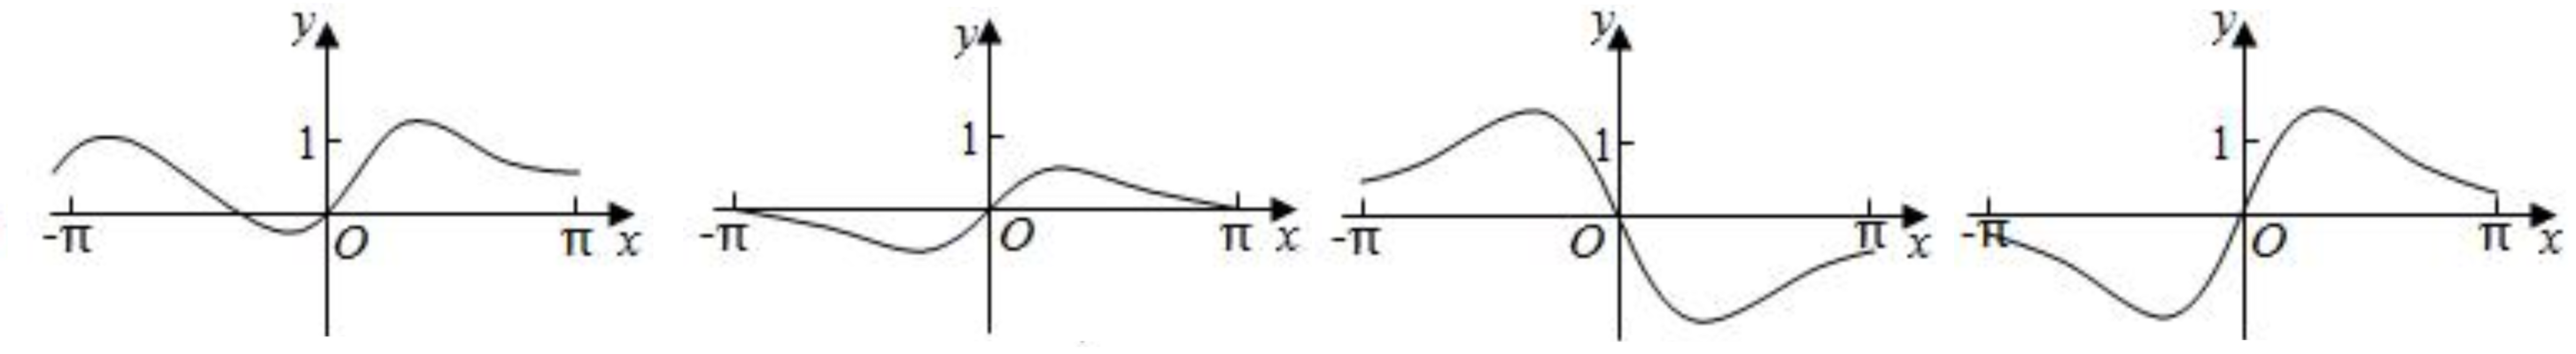
\includegraphics[width=12cm]{./F7UJfg6iYCiCefLftREhksYit6NP46Of.png}
\captionof{figure}{第5题}
\vspace{0.5cm}
\end{center}
\begin{solution}{4cm}

\end{solution}
\end{minipage}
\begin{minipage}{\textwidth}
\question[5] 某学校为了解$1000$名新生的身体素质,将这些学生编号为$1$,$2$,$ \cdots 1000$,从这些新生中用系统抽样方法等距抽取$100$名学生进行体质测试,若$46$号学生被抽到,则下面$4$名学生中被抽到的是\key{$C$}.


\fourchoices{$8$号学生}{$200$号学生}{$616$号学生}{$815$号学生 }
\begin{solution}{4cm}

\end{solution}
\end{minipage}
\begin{minipage}{\textwidth}
\question[5] $tan255^{\small \circ}=$\key{$D$}.
\fourchoices{$-2- \sqrt {3}$}{$-2+ \sqrt {3}$}{$2- \sqrt {3}$}{$2+ \sqrt {3}$}
\begin{solution}{4cm}

\end{solution}
\end{minipage}
\begin{minipage}{\textwidth}
\question[5]  已知非零向量$\overrightarrow{a}$,$\overrightarrow{b}$满足$|\overrightarrow{a}|=2|\overrightarrow{b}|$,且$(\overrightarrow{a}-\overrightarrow{b})\perp\overrightarrow{b}$,则$\overrightarrow{a}$与$\overrightarrow{b}$的夹角为\key{$B$}.
\fourchoices{$\dfrac{\pi}{6}$}{$\dfrac{\pi}{3}$}{$\dfrac{2\pi}{3}$}{$\dfrac{5\pi}{6}$ }
\begin{solution}{4cm}

\end{solution}
\end{minipage}
\begin{minipage}{\textwidth}
\question[5] 如图是求$\dfrac{1}{2+\dfrac{1}{2+\dfrac{1}{2}}}$的程序框图,图中空白框中应填入\key{$A$}.




\fourchoices{$A= \dfrac{1}{2+A}$}{$A= 2+\dfrac{1}{A}$}{$A= \dfrac{1}{1+2A}$}{$A= 1+\dfrac{1}{2A}$ }
\begin{center}
\write18{wget 'http://www.mathcrowd.cn/uploads/fig/lRyWbWTAbMoaIHdzGNbnHtHNwMC1OqLS.png'}
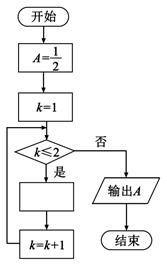
\includegraphics[width=4cm]{./lRyWbWTAbMoaIHdzGNbnHtHNwMC1OqLS.png}
\captionof{figure}{第9题}
\vspace{0.5cm}
\end{center}
\begin{solution}{4cm}

\end{solution}
\end{minipage}
\begin{minipage}{\textwidth}
\question[5] 双曲线$C$:$ \dfrac {x^{2}}{a^{2}} - \dfrac {y^{2}}{b^{2}} =1(a  \gt  0 , b  \gt  0)$的一条渐近线的倾斜角为$130^{\small \circ}$,则$C$的离心率为\key{$D$}.
\fourchoices{$2sin40^{\small \circ}$}{$2cos40^{\small \circ}$}{$ \dfrac {1}{sin50 ^\circ }$}{$ \dfrac {1}{cos50 ^\circ }$}
\begin{solution}{4cm}

\end{solution}
\end{minipage}
\begin{minipage}{\textwidth}
\question[5] $\triangle ABC$的内角$A$,$B$,$C$的对边分别为$a$,$b$,$c$,已知$asinA-bsinB=4csinC$,$cosA=- \dfrac {1}{4}$,则$ \dfrac {b}{c} =$\key{$A$}.
\fourchoices{$6$}{$5$}{$4$}{$3$}
\begin{solution}{4cm}

\end{solution}
\end{minipage}
\begin{minipage}{\textwidth}
\question[5] 已知椭圆$C$的焦点为${F}_{1}( - 1,0),{F}_{2}(1,0)$,过$F _{2}$的直线与$C$交于$A$,$B$两点$.$若$|A{F}_{2}|=2|{F}_{2}B|$,$|AB|=|B{F}_{1}|$,则$C$的方程为\key{$B$}.
\fourchoices{$\dfrac{{x}^{2}}{2}+{y}^{2}=1$}{$\dfrac{{x}^{2}}{3}+ \dfrac{{y}^{2}}{2}=1$}{$\dfrac{{x}^{2}}{4}+ \dfrac{{y}^{2}}{3}=1$}{$\dfrac{{x}^{2}}{5}+ \dfrac{{y}^{2}}{4}=1$}
\begin{solution}{4cm}

\end{solution}
\end{minipage}
\end{questions}
\group{填空题}{本大题共4小题,共20.0分}
\begin{questions}[]
\begin{minipage}{\textwidth}
\question[5]  曲线$y=3(x ^{2} +x)e ^{x}$在点$(0 , 0)$处的切线方程为\key{$y=3x$}.
\begin{solution}{4cm}

\end{solution}
\end{minipage}
\begin{minipage}{\textwidth}
\question[5]  记$S _{n}$为等比数列$\{a _{n} \}$的前$n$项和,若$a _{1} =1$,$S _{3} = \dfrac{3}{4}$,则$S _{4} =$\key{$ \dfrac {5}{8}$}.
\begin{solution}{4cm}

\end{solution}
\end{minipage}
\begin{minipage}{\textwidth}
\question[5]  函数$f(x)=\sin(2x+ \dfrac{3\pi}{2} )-3cosx$的最小值为\key{$-4$}.
\begin{solution}{4cm}

\end{solution}
\end{minipage}
\begin{minipage}{\textwidth}
\question[5] 已知$ \angle ACB=90^{\small \circ}$,$P$为平面$ABC$外一点,$PC=2$,点$P$到$ \angle ACB$两边$AC$,$BC$的距离均为$\sqrt{3}$,那么$P$到平面$ABC$的距离为\key{$ \sqrt {2}$}.
\begin{solution}{4cm}

\end{solution}
\end{minipage}
\end{questions}
\group{解答题}{本大题共7小题,共82.0分}
\begin{questions}[]
\begin{minipage}{\textwidth}
\question[12] 某商场为提高服务质量,随机调查了$50$名男顾客和$50$名女顾客,每位顾客对该商场的服务给出满意或不满意的评价,得到下面列联表:

\[\begin{array}{|l|l|l|}
\hline
 & \text{满意} & \text{不满意}\\
\hline
 \text{男顾客} & 40 & 10\\
\hline
 \text{女顾客} & 30 & 20\\
\hline
\end{array}\]
\begin{subquestions}
    \subquestion 分别估计男、女顾客对该商场服务满意的概率;
    \subquestion 能否有$95\%$的把握认为男、女顾客对该商场服务的评价有差异?

 附:${{K}^{2}}=\dfrac{n{{(ad-bc)}^{2}}}{(a+b)(c+d)(a+c)(b+d)}$.
 
 \[\begin{array}{|l|l|l|l|}
\hline
 P(K ^{2} \geqslant k) & 0.050 & 0.010 & 0.001\\
 \hline
 k & 3.841 & 6.635 & 10.828\\
 \hline
 \end{array}\]
\end{subquestions}
\begin{solution}{8cm}

\end{solution}
\end{minipage}
\begin{minipage}{\textwidth}
\question[12] 记$S _{n}$为等差数列$\{a _{n} \}$的前$n$项和,已知$S _{9} =-a _{5}$.$(1)$若$a _{3} =4$,求$\{a _{n} \}$的通项公式;$(2)$若$a _{1}  \gt  0$,求使得$S _{n} \geqslant a _{n}$的$n$的取值范围.
\begin{solution}{8cm}

\end{solution}
\end{minipage}
\begin{minipage}{\textwidth}
\question[12] 如图,直四棱柱$ABCD-A _{1} B _{1} C _{1} D _{1}$的底面是菱形,$AA _{1} =4$,$AB=2$,$ \angle BAD=60^{\small \circ}$,$E$,$M$,$N$分别是$BC$,$BB _{1}$,$A _{1} D$的中点.
\begin{subquestions}
    \subquestion 证明:$MN \parallel $平面$C _{1} DE$;
    \subquestion 求点$C$到平面$C _{1} DE$的距离.
\end{subquestions}
\begin{center}
\write18{wget 'http://www.mathcrowd.cn/uploads/fig/rOqrX8AOkhQtAGTSvgdyU0mzeH3pIfTp.png'}
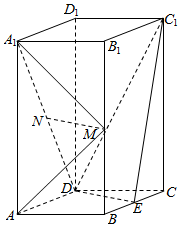
\includegraphics[width=4cm]{./rOqrX8AOkhQtAGTSvgdyU0mzeH3pIfTp.png}
\captionof{figure}{第19题}
\vspace{0.5cm}
\end{center}
\begin{solution}{8cm}

\end{solution}
\end{minipage}
\begin{minipage}{\textwidth}
\question[12] 已知函数$f(x)=2sinx-xcosx-x$,$f ' (x)$为$f(x)$的导数. $(1)$证明:$f ' (x)$在区间$(0 ,  \pi )$存在唯一零点; $(2)$若$x \in [0 ,  \pi ]$时,$f(x)\geqslant ax$,求$a$的取值范围.
\begin{solution}{8cm}

\end{solution}
\end{minipage}
\begin{minipage}{\textwidth}
\question[12] 已知点$A$,$B$关于坐标原点$O$对称,$|AB|=4$,$ \odot M$过点$A$,$B$且与直线$x+2=0$相切.
\begin{subquestions}
    \subquestion 若$A$在直线$x+y=0$上,求$ \odot M$的半径; 
    \subquestion 是否存在定点$P$,使得当$A$运动时,$|MA|-|MP|$为定值?并说明理由.
\end{subquestions}
\begin{solution}{8cm}

\end{solution}
\end{minipage}
\begin{minipage}{\textwidth}
\question[10] 在直角坐标系$xOy$中,曲线$C$的参数方程为$\left\{ \begin{matrix} x\text{=}\dfrac{1\text{-}t^{2}}{1\text{+}t^{2}}\text{,} \\ y\text{=}\dfrac{4t}{1\text{+}t^{2}} \\ \end{matrix} \right. (t$为参数$).$以坐标原点$O$为极点,$x$轴的正半轴为极轴建立极坐标系,直线$l$的极坐标方程为$2 \rho cos \theta + \sqrt{3}  \rho sin \theta +11=0$.
\begin{subquestions}
    \subquestion 求$C$和$l$的直角坐标方程; 
    \subquestion 求$C$上的点到$l$距离的最小值.
\end{subquestions}
\begin{solution}{8cm}

\end{solution}
\end{minipage}
\begin{minipage}{\textwidth}
\question[12] 已知$a$,$b$,$c$为正数,且满足$abc=1.$证明: 
\begin{subquestions}
    \subquestion $(1) \dfrac{1}{a} + \dfrac{1}{b} + \dfrac{1}{c} \leqslant a ^{2} +b ^{2} +c ^{2}$; 
    \subquestion $(2)(a+b) ^{3} +(b+c) ^{3} +(c+a) ^{3} \geqslant 24$.
\end{subquestions}
\begin{solution}{8cm}

\end{solution}
\end{minipage}
\end{questions}
\end{groups}
\label{lastpage}
\end{document}
